\documentclass[12pt]{scrartcl}

\usepackage{amsmath,amssymb}
\usepackage{fullpage}
\usepackage{hyperref}
\usepackage{graphicx}
\usepackage{tikz}
\usepackage[inline]{enumitem}
\usepackage{tabularx}
\usepackage{array}

\newcolumntype{Y}{>{\centering\arraybackslash}X}
\newcolumntype{L}[1]{>{\raggedright\arraybackslash}p{#1}}
\newcolumntype{C}[1]{>{\centering\arraybackslash}p{#1}}

\setlist[enumerate,1]{label=\alph*), itemjoin=\hspace{1.2em}, itemjoin*=\hspace{1.2em}}

\usetikzlibrary{calc}

\setlength{\parindent}{0pt}

\begin{document}

\begin{center}
	\hrule
	\vspace{0.4cm}
	{\textbf{\large Tutorial 01}}\\ [0.2cm]
	INF1004 Mathematics II

\end{center}

\textbf{Name:} Timothy Chia \hspace{\fill} \textbf{Date:} - \\

\hrule

\begin{enumerate}[label=\textbf{\arabic*.}]

	\item  In a sample of 20 people the times taken, in seconds, to solve a simple numerical puzzle
	      were as follows:

	      \begin{center}
		      \begin{tabular}{c c c c c c c c c c}
			      17 & 19 & 22 & 26 & 28 & 31 & 34 & 36 & 38 & 39 \\
			      41 & 42 & 43 & 47 & 50 & 51 & 53 & 55 & 57 & 58 \\
		      \end{tabular}
	      \end{center}

	      \begin{enumerate}[label=(\alph*)]
		      \item Calculate the mean and standard deviation of these times.
		      \item In fact, 23 people attempted to solve this puzzle. However, 3 of them failed to solve it within the allotted time of 60 seconds, taking 62, 65 and 97 seconds respectively.\\[0.5cm] Calculate the interquartile range (IQR) of the times taken by all 23 people.
		      \item Are there any outliers in the dataset?
	      \end{enumerate}

	      \medskip

	      \textbf{Solution.}
	      %------------------------------------------------------------
	      \newpage
	\item Consider the following tree diagram. \\ [0.2cm]

	      \noindent\makebox[\textwidth][c]{%  
		      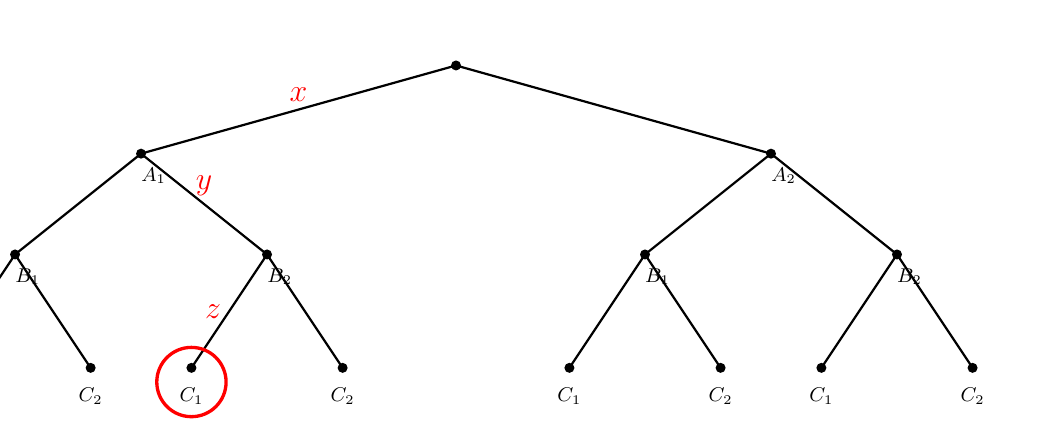
\begin{tikzpicture}[line cap=round, line join=round, thick, scale=0.80, transform shape]
			      \useasboundingbox (-6.8,-5.6) rectangle (9,0.6);
			      \tikzset{
				      dot/.style={circle, fill=black, inner sep=1.6pt},
				      lab/.style={font=\small},
				      redlab/.style={red, font=\Large\bfseries\itshape}
			      }

			      % --- coordinates (tweak if you want different spacing)
			      \coordinate (R)  at (0,0);

			      \coordinate (A1) at (-5,-1.4);
			      \coordinate (A2) at ( 5,-1.4);

			      \coordinate (B11) at (-7,-3.0);
			      \coordinate (B12) at (-3,-3.0);

			      \coordinate (C111) at (-8.2,-4.8);
			      \coordinate (C112) at (-5.8,-4.8);

			      \coordinate (C121) at (-4.2,-4.8); % this is the circled C1
			      \coordinate (C122) at (-1.8,-4.8);

			      \coordinate (B21) at ( 3,-3.0);
			      \coordinate (B22) at ( 7,-3.0);

			      \coordinate (C211) at ( 1.8,-4.8);
			      \coordinate (C212) at ( 4.2,-4.8);

			      \coordinate (C221) at ( 5.8,-4.8);
			      \coordinate (C222) at ( 8.2,-4.8);

			      % --- edges + red edge labels
			      \draw (R) -- (A1) node[midway, above, redlab] {$x$};
			      \draw (R) -- (A2);

			      \draw (A1) -- (B11);
			      \draw (A1) -- (B12) node[midway, above, redlab] {$y$};

			      \draw (B11) -- (C111);
			      \draw (B11) -- (C112);

			      \draw (B12) -- (C121) node[midway, left, redlab] {$z$};
			      \draw (B12) -- (C122);

			      \draw (A2) -- (B21);
			      \draw (A2) -- (B22);

			      \draw (B21) -- (C211);
			      \draw (B21) -- (C212);

			      \draw (B22) -- (C221);
			      \draw (B22) -- (C222);

			      % --- dots at all nodes
			      \node[dot] at (R)   {};
			      \node[dot] at (A1)  {};
			      \node[dot] at (A2)  {};

			      \node[dot] at (B11) {};
			      \node[dot] at (B12) {};
			      \node[dot] at (B21) {};
			      \node[dot] at (B22) {};

			      \node[dot] at (C111) {};
			      \node[dot] at (C112) {};
			      \node[dot] at (C121) {};
			      \node[dot] at (C122) {};

			      \node[dot] at (C211) {};
			      \node[dot] at (C212) {};
			      \node[dot] at (C221) {};
			      \node[dot] at (C222) {};

			      % --- labels near nodes (slightly offset to mimic the figure)
			      \node[lab] at ($(A1)+(0.20,-0.35)$) {$A_1$};
			      \node[lab] at ($(A2)+(0.20,-0.35)$) {$A_2$};

			      \node[lab] at ($(B11)+(0.20,-0.35)$) {$B_1$};
			      \node[lab] at ($(B12)+(0.20,-0.35)$) {$B_2$};
			      \node[lab] at ($(B21)+(0.20,-0.35)$) {$B_1$};
			      \node[lab] at ($(B22)+(0.20,-0.35)$) {$B_2$};

			      \node[lab] (c111lab) at ($(C111)+(0.00,-0.45)$) {$C_1$};
			      \node[lab] (c112lab) at ($(C112)+(0.00,-0.45)$) {$C_2$};

			      \node[lab] (c121lab) at ($(C121)+(0.00,-0.45)$) {$C_1$};
			      \node[lab] (c122lab) at ($(C122)+(0.00,-0.45)$) {$C_2$};

			      \node[lab] (c211lab) at ($(C211)+(0.00,-0.45)$) {$C_1$};
			      \node[lab] (c212lab) at ($(C212)+(0.00,-0.45)$) {$C_2$};

			      \node[lab] (c221lab) at ($(C221)+(0.00,-0.45)$) {$C_1$};
			      \node[lab] (c222lab) at ($(C222)+(0.00,-0.45)$) {$C_2$};

			      % --- red circle around the left-subtree C1 under B2
			      \draw[red, very thick]
			      ($(C121)!0.5!(c121lab)$) circle [radius=0.55];

		      \end{tikzpicture}
	      }

	      \begin{enumerate}[label=(\alph*)]
		      \item What does the probability $x$ represent?

		            \begin{enumerate*}[label=\alph*)]
			            \item $P(A_1)$ \quad \quad
			            \item $P(A_1 \mid B_2)$ \quad \quad
			            \item $P(B_2 \mid A_1)$ \quad \quad
			            \item $P(C_1 \mid B_2 \cap A_1)$ \quad \quad
		            \end{enumerate*}

		            \medskip

		      \item What does the probability $y$ represent?

		            \begin{enumerate*}[label=\alph*)]
			            \item $P(B_2)$ \quad \quad
			            \item $P(A_1\mid B_2)$ \quad \quad
			            \item $P(B_2\mid A_1)$ \quad \quad
			            \item $P(C_1\mid B_2 \cap A_1)$ \quad \quad
		            \end{enumerate*}

		            \medskip

		      \item The probability $z$ represents?

		            \begin{enumerate*}[label=\alph*)]
			            \item $P(C_1)$ \quad \quad
			            \item $P(B_2\mid C_1)$ \quad \quad
			            \item $P(C_1\mid B_2)$ \quad \quad
			            \item $P(C_1\mid B_2 \cap A_1)$ \quad \quad
		            \end{enumerate*}

		            \medskip

		      \item The circled node represents the event?

		            \begin{enumerate*}[label=\alph*)]
			            \item $C_1$ \quad \quad
			            \item $B_2 \cap C_1$ \quad \quad
			            \item $A_1 \cap B_2 \cap C_1$ \quad \quad
			            \item $C_1 \mid (B_2 \cap A_2)$ \quad \quad
		            \end{enumerate*}

		            \medskip

		      \item Let $A$ and $B$ be two events. Suppose that the probability that neither event occurs is $\tfrac{3}{8}$.
		            What is the probability that at least one of the events occurs?

		            \medskip

		      \item Let $C$ and $D$ be two events. Suppose $P(C)=0.5$, $P(C\cap D)=0.2$ and $P\big((C\cup D)^c\big)=0.4$.
		            What is $P(D)$?
	      \end{enumerate}

	      \medskip

	      \textbf{Solution.}


	      %------------------------------------------------------------
	      \newpage
	\item In a survey of 1929 students, the following data were obtained on ``students' first reason
	      for application to the university in which they matriculated.''

	      \medskip

	      \begin{center}
		      \small
		      \setlength{\tabcolsep}{6pt}
		      \renewcommand{\arraystretch}{1.2}

		      \begin{tabular}{p{0.25\linewidth}|c c c|c}
			      \textbf{Enrollment status} &
			      \textbf{\shortstack{University                      \\Quality}} &
			      \textbf{\shortstack{University Cost                 \\or Convenience}} &
			      \textbf{Other}             &
			      \textbf{Total}                                      \\
			      \hline
			      Full-time                  & 421 & 393 & 76  & 890  \\
			      Part-time                  & 400 & 593 & 46  & 1039 \\
			      \hline
			      Total                      & 821 & 986 & 122 & 1929 \\
		      \end{tabular}
	      \end{center}

	      \medskip

	      \begin{enumerate}[label=(\alph*)]
		      \item What is the probability that university quality is the first reason for a student to choose a university?
		      \item For a full-time student, what is the probability that university quality is the first reason for choosing a university?
		      \item Let $A$ denote the event that a student is full-time, and let $B$ denote the event that the student
		            lists university quality as the first reason for applying. Are events $A$ and $B$ independent?
	      \end{enumerate}

	      \medskip

	      \textbf{Solution.}

	      %------------------------------------------------------------
	      \newpage
	\item A rare blood disease is found in 2\% of a certain population. A new blood test can correctly
	      identify 96\% of the people with the disease and 94\% of the people without the disease.

	      \begin{enumerate}[label=(\alph*)]
		      \item What is the probability that a person who is tested positive by the blood test actually has the disease?
		      \item What is the probability that a person who is tested negative by the blood test actually does not have the disease?
	      \end{enumerate}

	      \medskip

	      \textbf{Solution.}

	      %------------------------------------------------------------
	      \newpage
	\item A woman is pregnant with male twins. Twins may be either identical or fraternal (non-identical).
	      In general, $\tfrac{1}{3}$ twins born are identical. Obviously, identical twins must be of the same sex;
	      fraternal twins may or may not be. Assume that identical twins are equally likely to be both boys or both girls,
	      while for fraternal twins all possibilities are equally likely: boy-girl, girl-boy, boy-boy, girl-girl.
	      Given the above information, what is the probability that the woman's male twins are identical?

	      \medskip
	      \textbf{Solution.}

	      %------------------------------------------------------------
	      \newpage
	\item If a family had three kids, named Alice, Bob, and Carl. Assume that each is equally likely to be born;
	      i.e., $1/3$ chance for each of them to be born first etc.

	      \begin{enumerate}[label=(\alph*)]
		      \item Find the probability that Alice is older than Bob, given that Alice is older than Carl.
		      \item Is event ``Alice is older than Bob'' independent from event ``Alice is older than C''?
	      \end{enumerate}

	      \medskip

	      \textbf{Solution.}

	      %------------------------------------------------------------
	      \newpage
	\item A boy receives a school report card each week. He is given a special treat whenever his report indicates
	      ``Good behavior'' \textbf{AND} ``Excellent Homework''. His behavior is good with probability 0.6.
	      When his behavior is good, he has a probability of 0.8 of doing excellent homework. When his behavior is not good,
	      his probability of doing excellent homework is only 0.5.

	      \begin{enumerate}[label=(\alph*)]
		      \item For a random week, calculate the probability that he will be given a special treat.
		      \item For a random week, calculate the probability that his homework will be excellent but he will not be given a special treat.
		      \item For a random week, calculate the probability that his homework will be excellent.
		      \item Given that his homework is excellent, calculate the conditional probability that he is \textbf{NOT} given a special treat.
	      \end{enumerate}

	      \medskip

	      \textbf{Solution.}


	      %------------------------------------------------------------
	      \newpage
	\item In an attempt to find the mean number of hours his tutorial classmates spent per day preparing for tutorials,
	      John collected data from 10 of his friends in the tutorial group and found that the sample mean is 2.4 hours with a
	      sample standard deviation of 0.8 hours. However, a day later he felt that the sample size is too small.
	      So he collected data from another 5 of his friends and found that the sample mean is 2.0 hours with a sample
	      standard deviation of 1.2 hours.

	      \medskip

	      Find the sample mean and sample standard deviation \underline{when these 2 sets of data are combined}.

	      \medskip
	      \textbf{Solution.}

	      %------------------------------------------------------------
	      \newpage
	\item A certain family has 6 children, consisting of 3 boys and 3 girls. Assuming that all birth orders are equally likely,
	      what is the probability that the 3 eldest children are the 3 girls?

	      \medskip
	      \textbf{Solution.}

\end{enumerate}

\end{document}
